\documentclass[12pt, a4paper]{article}
\usepackage{amsmath,amssymb}
\usepackage{amsthm}
\usepackage{xcolor}
\usepackage[margin=0.25in]{geometry}
\usepackage{pgfplots}
\pgfplotsset{width=10cm,compat=1.9}
\title{Analisi I}
\newtheoremstyle{break}
  {\topsep}{\topsep}%
  {\itshape}{}%
  {\bfseries}{}%
  {\newline}{}%
\theoremstyle{break}
\newtheorem{theorem}{Teorema}[subsection]
\newtheorem{corollary}{Corollario}[theorem]
\newtheorem{lemma}[theorem]{Lemma}
\newtheorem{definition}{Definizione}[subsection]
\newtheorem{proposition}{Proposizione}[subsection]
\newtheorem{example}{Esempio}[subsection]
\newtheorem{observation}{Osservazione}[subsection]

\newcommand\R{{\rm I\!R}}
\newcommand\Rext{\overline{\R}}
\newcommand{\Lim}[3]{\lim_{#1} #2 = #3}
%\newcommand\func[3]{#1:#2\rightarrow #3}
\newcommand{\func}[3]{#1:#2\rightarrow #3}
\newenvironment{plot}{
    \begin{figure}[!htb]
        \centering
        \begin{tikzpicture}
}
{    
        \end{tikzpicture}
    \end{figure}
}
\author{Scannagatti Gabriele}
\begin{document}
\maketitle
\newpage
    \section{Insiemi Numerici}
    \begin{itemize}
        \item ${\rm I\!N}$ Insieme dei numeri naturali
        \item ${\rm \!Z}$ Insieme dei numeri interi positivi e negativi
        \item ${\rm \!Q}$ Insieme dei numeri razionali "frazioni"
        \item $\R$ Insieme dei numeri reali
    \end{itemize}
    \section{Intervalli}
    \begin{definition}
        $I\subset \R$ si dice intervallo se $\forall x,y\in I.\,(x<y\Rightarrow \exists z\in \R.(x<z<y\Rightarrow z\in I))$
        \newline
        In un intervallo "non ci sono buchi".
    \end{definition}
    \begin{example}
        $A = \{x\in \R :\, 2<x<3\}$ è un intervallo \newline
        $B = \{x\in \R: 1\leq x < 2\, \vee\, 5<x\leq6\}$ non è un intervallo        
    \end{example}
    \subsection{Notazione}
    dati $a,b\in \R.\quad a<b$ allora:
    \begin{itemize}
        \item $[a,b] = \{x\in\R:\quad a\leq x\leq b\}$ intervallo chiuso.
        \item $(a,b) = \{x\in\R:\quad a<x<b\}$ intervallo aperto.
        \item $(a,b] = \{x\in\R:\quad a<x\leq b\}$ intervallo aperto a sx e chiuso a dx (si può avere anche il viceversa).
        \item $[a,+\infty) = \{x\in\R:\quad x\geq a\}$ semiretta chiusa.
        \item $(a, +\infty) = \{x\in\R:\quad x > a\}$ semiretta aperta.
        \item $(-\infty,+\infty) = \R$
    \end{itemize}
    \newpage
    \section{Funzioni}
    \begin{definition}
        Una funzione $f$ è una terna di oggetti: $A,\,B,\,f$ di cui $A,\,B$ insiemi per cui:\newline
        $A$ si dice dominio, $B$ si dice codominio ed $f$ è una relazione che lega gli elementi di $A$ a quelli di $B$.
        \[f:A\rightarrow B\]
        In particolare: $f$ è una relazione totale ed univalente \scriptsize \textbf{(vedi definizioni di fondamenti dell'informatica)}
        \normalsize
    \end{definition}
    \subsection{Grafico di $f$}
    il grafico di una funzione $f$ è definito dall'insieme:
    \[f: A\rightarrow B\quad Graph(f) = \{(a,b)\in A\times B\,:\quad b = f(a)\}\]
    \begin{example}
        \begin{figure}[!htb]
            \centering
            \begin{tikzpicture}
                \begin{axis}[
                    axis lines = middle,
                    xmin = -2,
                    xmax = 2,
                    ymin = 0,
                    ymax = 2,
                    samples = 100
                ]
                \addplot[blue] {x^2};
                \end{axis}
            \end{tikzpicture} 
        \end{figure}
    \end{example}
    \subsection{Immagine di $f$}
    $f: A\rightarrow B$ funzione, $D\subset A \quad f(D) = \{f(x) :\; x\in D\}$ si dice immagine di D attraverso $f$ e
    $f(D)\subset B$. \newline $Imm(f) = f(A)$ immagine di $f$ ovvero l'immagine di tutto il dominio attraverso $f$.
    \newline
    \begin{example}
        \[A,\,B = \R\quad f(x) = x^2\quad D = [1,3]\quad f(D) = [1,9]\]
        \[Imm(f) = f(A) = f(\R) = [0, +\infty)\]
    \end{example}
    \newpage
    \subsection{Funzioni iniettive, surgettive e bigettive}
    \begin{definition}
        Una funzione $f: A\rightarrow B$ si dice surgettiva se: $\forall y\in B.\; \exists x\in A.\; y = f(x)$, 
    \end{definition}
    quindi ad esempio $f(x) = x^2\quad g(x) = x^3$ entrambe definite in $\R^2$ abbiamo che: $f$ non è surgettiva (per $y=-4$ non esiste alcun $x$ tale che $f(x) = -4$), mentre $g$ è surgettiva.
    \begin{observation}
        $f:A\rightarrow B$ è surgettiva $\Leftrightarrow$ $Imm(f) = B$
    \end{observation}
    \begin{definition}
        Una funzione $f:A\rightarrow B$ si dice iniettiva se: $\forall x_1,\,x_2\in A.\; f(x_1) \neq f(x_2)$,
    \end{definition}
    quindi ad esempio $f(x) = x^2\quad g(x) = x^3$ entrambe definite in $\R^2$ abbiamo che: $f$ non è iniettiva in quanto \newline$x_1 = 2,\, x_2 = -2\; f(x_1) = f(x_2) = 4$, mentre $g$ è iniettiva.
    \begin{definition}
        Una funzione $f: A\rightarrow B$ si dice bigettiva (biunivoca, biiezione, invertibile) se: 
    \end{definition}
    $f$ è sia \textbf{iniettiva}, sia \textbf{surgettiva}. Se una funzione $f$ è bigettiva posso costruire la funzione inversa indicata come $f^{-1}: B\rightarrow A$. Dato $b\in B$ esiste almeno un elemento $a\in A$ tale che $f(a) = b$ ($f$ è surgettiva), inoltre l'elemento $a$ è unico perché $f$ è iniettiva.\newline
    Quindi $f^{-1}(b) = a \Leftrightarrow f(a) = b$.
    \begin{example}
        $f:[0, +\infty]\rightarrow [0,+\infty]\quad f(x) = x^2$ è bigettiva e la sua inversa è la radice quadrata:\newline
        $f^{-1}:[0,+\infty]\rightarrow [0,+\infty]\quad f^{-1}(y) = \sqrt{y}$.\newline
        La radice quadrata è la funzione inversa di $f(x)  = x^2$ quando dominio e codominio sono $[0,+\infty]$,\newline
        $\sqrt{y}$ è sempre un numero $\geq 0$.\newline
        \textbf{Osservazione:} $\sqrt{x^2} = |x|\quad x=-2\;\rightarrow \sqrt{(-2)^2} = \sqrt{4} = 2\quad x\neq 2\; |x| = 2$    
    \end{example}
    \subsection{Traslazioni di $f$}
    Se $g(x) = f(x) + \alpha\quad \alpha\in\R$ abbiamo una traslazione in verticale 
    $\left\{
        \begin{matrix}
            \text{Verso l'alto} \Rightarrow \alpha > 0 \\
            \text{Verso il basso} \Rightarrow \alpha < 0 \\
        \end{matrix}
    \right.$
    \newline
    \newline Se $g(x) = f(x + \alpha)\quad\alpha\in\R$ abbiamo una traslazione orizzontale
    $\left\{
        \begin{matrix}
            \text{Verso Sx}\Rightarrow \alpha > 0 \\
            \text{Verso Dx}\Rightarrow \alpha < 0 \\
        \end{matrix}
    \right.$
    \begin{figure}[!htb]
        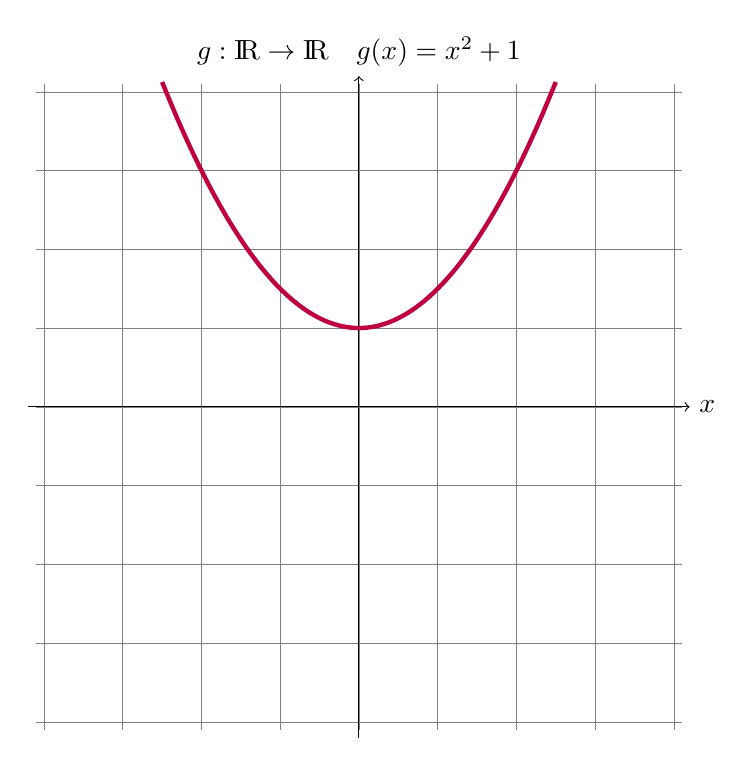
\begin{tikzpicture}
            \begin{scope}[xshift=9cm]
                \draw[very thin,color=gray] (-4.1,-4.1) grid (4.1,4.1);
                \draw[->] (-4.2,0) -- (4.2,0) node[right] {$x$};
                \draw[->] (0,-4.2) -- (0,4.2) node[above] {$g:\R \rightarrow \R\quad g(x) = x^2 + 1$};
        
                \draw[ultra thick,purple,domain=-2.5:2.5,smooth] plot (\x,{0.5*(\x)^2 + 1});
            \end{scope}
        \end{tikzpicture}
        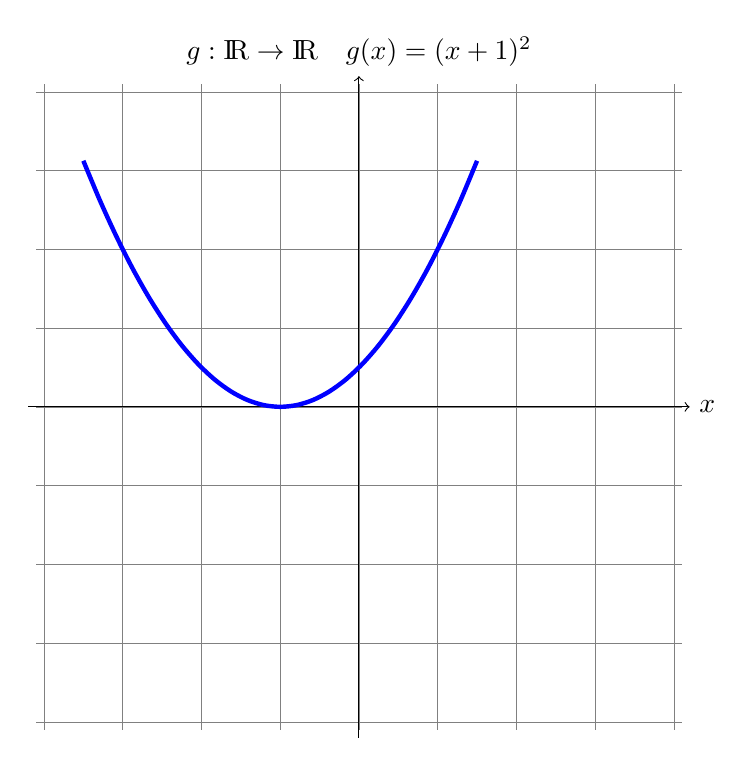
\begin{tikzpicture}
            \begin{scope}[xshift=9cm]
                \draw[very thin,color=gray] (-4.1,-4.1) grid (4.1,4.1);
                \draw[->] (-4.2,0) -- (4.2,0) node[right] {$x$};
                \draw[->] (0,-4.2) -- (0,4.2) node[above] {$g:\R \rightarrow \R\quad g(x) = (x+1)^2$};
        
                \draw[ultra thick,blue,domain=-3.5:1.5,smooth] plot (\x,{0.5*(\x + 1)^2});
            \end{scope}
        \end{tikzpicture}
    \end{figure}
    \newpage
    \subsection{Funzioni monotone}
    \subsubsection{Definizione}
    Data una funzione $f:A\rightarrow B\quad x_1,\,x_2\in A \wedge x_1<x_2$ abbiamo:
    \begin{enumerate}
        \item Se $f(x_1)<f(x_2),\, \forall x_1,\,x_2\; f$ é strettamente crescente.
        \item Se $f(x_1)\leq f(x_2),\, \forall x_1,\,x_2\; f$ é debolmente crescente.
        \item Se $f(x_1)>f(x_2),\, \forall x_1,\,x_2\; f$ é strettamente decrescente.
        \item Se $f(x_1)\geq f(x_2),\, \forall x_1,\,x_2\; f$ é debolmente decrescente.
        \item Se si verificano 1 o 3 $f$ é strettamente monotona.
        \item Se si verificano 2 o 4 $f$ é debolmente monotona.
    \end{enumerate}
    Se $f$ è crescente mantiene l'ordinamento, se $f$ è decrescente inverte l'ordinamento.
    \subsubsection{Rapporto incrementale e monotonia}
    \begin{definition}
        $f$ è strettamente crescente $\Leftrightarrow$ il suo rapporto incrementale $\frac{f(x_1)-f(x_2)}{x_1-x_2}$ è $> 0\quad \forall x_1,\,x_2. x_1\neq x_2$.
    \end{definition}
    \begin{definition}
        $f$ è strettamente decrescente $\Leftrightarrow$ il suo rapporto incrementale $\frac{f(x_1) - f(x_2)}{x_1-x_2}$ è $< 0\quad \forall x_1,\,x_2. x_1\neq x_2$.
    \end{definition}
    Analogamente se:
    \begin{itemize}
        \item $\frac{f(x_1)-f(x_2)}{x_1-x_2} \leq 0\Leftrightarrow f$ è debolmente decrescente.  
        \item $\frac{f(x_1)-f(x_2)}{x_1-x_2} \geq 0\Leftrightarrow f$ è debolmente crescente. 
    \end{itemize}
    \begin{example}
        $f(x) = \frac{1}{x},\; f:\R-\{0\} \rightarrow \R-\{0\}$ la funzione non è globalmente decrescente, \newline
        ma lo è sui due Intervalli
        $\left\{
            \begin{matrix}
                (-\infty, 0) \\
                (0,+\infty) \\
            \end{matrix}
        \right.$
    \end{example}
    \begin{figure}[!htb]
        \centering
        \begin{tikzpicture}
            \begin{axis}[
              axis lines=middle,
              samples=30,
            ]
            \addplot[red,domain=-3:-0.1] {0.5*(1/(x)) };
            \addplot[red,domain=0.1:3] {0.5*(1/(x)) };
            \end{axis}
        \end{tikzpicture}
    \end{figure}
    \newpage
    \subsection{Composizione di funzioni monotone}
    presi gli insiemi $A,B,C\subset\R\text{ e le funzioni }f:A\rightarrow B,\; g:B\rightarrow C$ risulta che:
    \begin{itemize}
        \item Se $f$ è crescente e $g$ è crescente $\Rightarrow\; g\circ f$ è crescente. 
        \item Se $f$ è crescente e $g$ è decrescente $\Rightarrow\; g\circ f$ è decrescente. 
        \item Se $f$ è decrescente e $g$ è crescente $\Rightarrow\; g\circ f$ è decrescente. 
        \item Se $f$ è decrescente e $g$ è decrescente $\Rightarrow\; g\circ f$ è crescente. 
    \end{itemize}
    \begin{observation}
        Se $f$ è strettamente monotona $\Rightarrow\; f$ è iniettiva. Il viceversa \textbf{non} vale.
    \end{observation}
    \subsection{Altre definizioni per funzioni ($f:A\rightarrow B$)}
    \begin{definition}
        L'insieme di definizione (o dominio naturale) di una funzione è il più grande sottoinsieme di $\R$ dove ha senso scrivere la funzione.
    \end{definition}
    \begin{definition}
        $f(x) \text{ è pari }\Leftrightarrow \forall x\in A.\; f(x) = f(-x)$
    \end{definition}
    \begin{definition}
        $f(x) \text{ è dispari }\Leftrightarrow \forall x\in A.\; f(x) = -f(x)$   
    \end{definition}
    \begin{observation}
        Per essere pari o dispari, una funzione ha bisogno di un dominio tale che $x\in A \wedge -x\in A$, ossia simmetrico rispetto all'origine.
        \begin{itemize}
            \item$f$ è pari $\Rightarrow Graph(f)$ è simmetrico rispetto all'asse $y$.
            \item$f$ è dispari $\Rightarrow Graph(f)$ è simmetrico rispetto all'asse $x$.
            \item$f$ è periodica di periodo $\rho \Leftrightarrow \forall x\in A.\,(\forall c\in Z.\,(f(x) = f(x+c\rho)))$        
        \end{itemize}
    \end{observation}
    \begin{observation}
        Se $f$ è periodica o $f$ è pari allora $f$ non è monotona e f non è iniettiva.
        \begin{itemize}
            \item $x^\alpha = e^{\alpha log(x)}\quad\forall x > 0$
        \end{itemize}
    \end{observation}
    \section{Massimi e Minimi}
    \begin{definition}
        $A\subset\R,\; A\neq\emptyset,\; m\in\R$ si dice massimo di A se $m\geq a,\; \forall a\in A \wedge m \in A$.
    \end{definition}
    \begin{definition}
        $A\subset\R,\; A\neq\emptyset,\; m\in\R$ si dice minimo di A se $m\leq a,\; \forall a\in A \wedge m \in A$. 
    \end{definition}
    \begin{observation}
        Se $A = [x,y)$ è un intervallo aperto a dx allora non ha massimo.
        \begin{proof}
            Supponendo per assurdo che $m\in\R$ sia il $max(A)$, allora $m\in A \wedge m<y$ perché $y$ è escluso.\newline
            Ponendo $\varepsilon = y-m > 0$, definiamo $m' = m + \frac{\varepsilon}{2}$.\newline 
            Risulta quindi che $m' \in A$, ma $m' > m$ contraddicendo la definizione.
        \end{proof}
    \end{observation}
    \begin{observation}
        Analogamente se $A = (x,y]$ allora non ha minimo
    \end{observation}
    \section{Maggioranti e Minoranti}
    \begin{definition}
        $A\subset\R,\; A\neq\emptyset,\; k\in\R$ si dice maggiorante di $A$ se $k\geq a\; \forall a \in A$. L'insieme dei maggioranti di $A$ si indica con $M_A$.
        \begin{observation}
            Se esiste un maggiorante di $A$, allora ne esistono infiniti.\newline
            non tutti gli insiemi hanno maggioranti, ad esempio $B = [0,+\infty)$ non ha maggiorante
        \end{observation}
    \end{definition}
    \begin{definition}
        Se l'insieme $M_A\neq\emptyset\Rightarrow A$ si dice superiormente limitato e $Sup(A) = min(M_A)$. 
    \end{definition}
    \begin{observation}
        Le defenizioni per i Minoranti sono analoghe alle precedenti.
    \end{observation}
    \begin{definition}
    Se $A$ è sia superiormente limitato, sia inferiormente limitato, allora $A$ si dice limitato.
    \end{definition}
    \begin{theorem}
        $A\subset\R,\; A\neq\emptyset,\, A$ è superiormente limitato $\Rightarrow\exists\, min(M_A)$ tale minimo si dice estremo superiore di $A\; Sup(A)$.
    \end{theorem}
    \section{Retta reale estesa}
    \subsubsection{Definizione}
    La retta reale estesa $\overline{\R} = \R \cup \{-\infty\}\cup\{+\infty\}$ in modo che valga:
    \[-\infty \leq x \leq +\infty\quad\forall x\in\overline{\R}\]
    \begin{observation}
        Se $x\in\R$ allora $-\infty<x<+\infty$
    \end{observation}
    \subsubsection{Operazioni in $\overline{\R}$}
    \begin{enumerate}
        \item Se $x\neq+\infty\Rightarrow x+(-\infty) = -\infty$
        \item Se $x\neq-\infty\Rightarrow x+(+\infty) = +\infty$
        \item Se $x > 0\Rightarrow x*(+\infty) = +\infty \wedge x*(-\infty) = -\infty$
        \item Se $x < 0\Rightarrow x*(+\infty) = -\infty \wedge x*(-\infty) = +\infty$
    \end{enumerate}
    \subsubsection{Operazioni Vietate}
    \begin{enumerate}
        \color{red}
        \item $(+\infty) + (-\infty)$ e viceversa
        \item $0*(+\infty)$
        \item $0*(-\infty)$ 
    \end{enumerate}
    \subsubsection{Operazioni valide}
    \begin{enumerate}
        \item $(+\infty)*(+\infty) = +\infty$
        \item $(+\infty)*(-\infty) = -\infty$ e viceversa
        \item $(-\infty)*(-\infty) = +\infty$
    \end{enumerate}
    \newpage
    \begin{observation}
        Dato $A\subset Z$ se $A$ è superiormente limitato allora $A$ ha massimo e se $A$ è inferiormente limitato
        allora $A$ ha minimo.
    \end{observation}
    \begin{definition}
        Dato $x\in\R$ si dice parte intera di $x$ e si indica con $[x]$ il numero $[x] = max(m\in Z :\; m\leq x)$
    \end{definition}
    \begin{example}
        $\left[\frac{25}{10}\right]=2$\newline\newline
        Graficamente:
    \end{example}
    \begin{figure}[!htb]
        \centering
        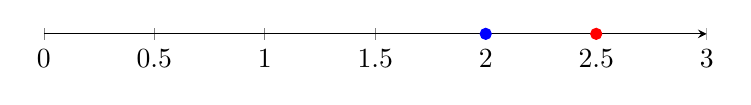
\begin{tikzpicture}
            \begin{axis}[
              axis x line=middle,
              axis y line = none,
              xmin=0,
              xmax=3,
            ]
            \addplot[red, only marks] 
            table {
                2.5 0
            };
            \addplot[blue, only marks]
            table {
                2 0
            };
            \end{axis}
        \end{tikzpicture}
    \end{figure}
    \begin{example}
        Grafico di $f(x)=[x]$
    \end{example}
    \begin{figure}[!htb]
        \centering
        \begin{tikzpicture}
            \begin{axis}[
              axis lines=middle,
              xmin=0,
              xmax=5
            ]
            \addplot[red] coordinates {(0,0) (0.95,0)};
            \addplot[red] coordinates {(1,1) (1.95,1)};
            \addplot[red] coordinates {(2,2) (2.95,2)};
            \addplot[red] coordinates {(3,3) (3.95,3)};
            \addplot[red] coordinates {(4,4) (4.95,4)};
            \addplot[red] coordinates {(5,5) (5.95,5)};
            \end{axis}
        \end{tikzpicture}
    \end{figure}
    \section{Massimi e Minimi di $f$}
    \begin{definition}
        Dati $A\subset\R,\quad f:A\rightarrow \R$ $f$ si dice limitata superiormente se $f(A)$ è limitato superiormente.\newline 
        Analogamente $f$ è inferiormente limitata se $f(A)$ è limitato inferiormente.
    \end{definition}
    \begin{definition}
        $f$ ha massimo se $f(A)$ ha massimo, si dice che $M$ è il massimo di $f$ e si indica con $M = max(f)$.\newline
        Analogamente per il minimo indicato con $min(f)$.
    \end{definition}
    \begin{definition}
        L'estremo superiore di una funzione è uguale a $sup(f) = sup(f(A))$, se $f$ non è limitata superiormente si indica $sup(f) = +\infty$, nel caso non sia inferiormente limitata si indica con $inf(f)  = -\infty$.
    \end{definition}
    \begin{definition}
        Se $f$ ha massimo allora $\forall x_0\in A.\; f(x_0) = max(f)) \Rightarrow x_0$ si dice punto di massimo, stessa cosa per i punti di minimo.
    \end{definition}
    \begin{observation}
        Il massimo di $f$ è unico, i punti di massimo potrebbero essere molti
    \end{observation}
    \newpage
    \begin{example}
        $f:\R\rightarrow\R\; f(x) = \sin(x)\quad max(f) = 1\; x_0 = \frac{\pi}{2}+2k\pi,\, k\in Z$ sono punti di massimo.
    \end{example}
    \begin{figure}[!htb]
        \centering
        \begin{tikzpicture}
            \begin{axis}[
                axis lines = middle,
                xmin = -10,
                xmax = 10,
                ymin = -3,
                ymax = 3, 
                trig format plots=rad,
                samples=100
            ]

            \addplot[red, domain=-10:10] {sin(x)};
            \addplot[blue, dashed] coordinates {(0,1) (3.14/2, 1)};
            \addplot[blue, dashed] coordinates {(3.14/2, 0) (3.14/2,1)};
                
            \end{axis}
        \end{tikzpicture}
    \end{figure}
    \begin{example}
        $f:(0,+\infty)\rightarrow\R\; f(x) = \frac{1}{x}\quad f$ non ha nè massimo nè minimo.
    \end{example}
    \begin{figure}[!htb]
        \centering
        \begin{tikzpicture}
            \begin{axis}[
                axis lines = middle,
                xmin = -1,
                xmax = 5,
                ymin = -1,
                ymax = 4,
                samples = 100
            ]
            \addplot[black, domain=0.1:10] {1/x};
            \addplot[red] coordinates {(-1,2)(5,2)};
            \addplot[red, dashed] coordinates {(1/2,2)(1/2,0)};
            \addplot[blue] coordinates {(-1,1/3)(5,1/3)};
            \end{axis}
        \end{tikzpicture}
    \end{figure}
    \newpage
    \begin{observation}
        Presi $A\subset{}\rm I\!R,\; f:A\rightarrow\R$ si ha che:
        \begin{itemize}
            \item Se $A$ ha massimo e $f$ è debolmente crescente, allora $f$ ha max e $max(f) = f(max(A))$.
            \item Se $A$ ha minimo e $f$ è debolmente crescente, allora $f$ ha min e $min(f) = f(min(A))$.
            \item Se $A$ ha massimo e $f$ è debolmente decrescente, allora $f$ ha min e $min(f) = f(max(A))$.
            \item Se $A$ ha minimo e $f$ è debolmente decrescente, allora $f$ ha max e $max(f) = f(min(A))$.
        \end{itemize}
    \end{observation}
    \begin{figure}[!htb]
        \begin{tikzpicture}
            \begin{axis}[
                axis lines = middle,
                xmin = 0,
                xmax = 5,
                ymin = 0,
                ymax = 4,
                samples = 100
            ]
            \addplot[black, domain=1:4] {ln(x)+1};
            \addplot[blue, dashed] coordinates {(1,0)(1,1)};
            \addplot[blue, dashed] coordinates {(0,1)(1,1)};
            \addplot[red, dashed] coordinates {(4,0)(4, 2.39)};
            \addplot[red, dashed] coordinates {(0, 2.39)(4,2.39)};
            \end{axis}
        \end{tikzpicture}
        \begin{tikzpicture}
            \begin{axis}[
                axis lines = middle,
                xmin = 0,
                xmax = 5,
                ymin = 0,
                ymax = 5,
                samples = 100
            ]
            \addplot[black, domain=1:4] {1/((1/2)*x) + 1};
            \addplot[red, dashed] coordinates {(1,0)(1,3)};
            \addplot[red, dashed] coordinates {(0,3)(1,3)}; 
            \addplot[blue, dashed] coordinates {(4,0)(4,1.5)};
            \addplot[blue, dashed] coordinates {(0,1.5)(4,1.5)};
            \end{axis}
        \end{tikzpicture}
    \end{figure}
    \begin{observation}
        $f:A\rightarrow \R$ allora $m = sup(f) \Leftrightarrow$ valgono le seguenti condizioni:
        \begin{enumerate}
            \item $f(x)\leq m\;\forall x\in A$
            \item $\forall\varepsilon > 0.\;\exists\overline{x}.\;f(\overline{x})>m-\varepsilon$
        \end{enumerate}
    \end{observation}
    \begin{figure}[!htb]
        \centering
        \begin{tikzpicture}
            \begin{axis}[
                axis lines = middle,
                xmin = 0,
                xmax = 10,
                ymin = 0,
                ymax = 2,
                samples = 100
            ]
            \addplot[black, domain=0.1:20] {(1-e^(-x/2))-0.05};
            \addplot[red] coordinates {(0,1)(10,1)};
            \node [red] at (5,110) {$m$};
            \addplot[blue,dashed] coordinates {(6,0)(6,0.9)};
            \node[blue] at (65,10) {$\overline{x}$};
            \addplot[blue,dashed] coordinates {(0,0.9)(6,0.9)};
            \node[blue] at (5,80) {$f(\overline{x})$};
            \addplot[purple] coordinates {(0,0.6)(10,0.6)};
            \node[purple] at (7,55) {$m-\varepsilon$};
            \end{axis}
        \end{tikzpicture}
    \end{figure}
    \newpage
    \section{Valore assoluto}
    \begin{definition}
        Dato $x\in\R$ si dice valore assoluto di $x$ e si indica con $|x|$ il numero $|x| = max(-x,x)$
    \end{definition}
    \subsubsection{Propietà del valore assoluto:}
    \begin{enumerate}
        \item $x\leq |x|\;\forall x\in\R$
        \item $|x| = x \Rightarrow x\geq0,\quad |x| = -x \Rightarrow x\leq0$
        \item $|x| = 0 \Leftrightarrow x = 0$
        \item $|-x| = |x|$
        \item $-|x|\leq x\leq |x|$
        \item $|x|\leq m \Leftrightarrow -m\leq x\leq m\quad (m\geq0)$
    \end{enumerate}
    \begin{figure}[!htb]
        \centering
        \begin{tikzpicture}
            \begin{axis}[
                axis lines = middle,
                xmin = -5,
                xmax = 5,
                ymin = 0,
                ymax = 5,
                samples = 100
            ]
            \addplot[blue] {abs(x)};
            \addplot[red] coordinates {(-5,3)(5,3)};
            \node[red] at (550,325) {$m$};
            \addplot[red, dashed] coordinates {(-3,3)(-3,0)};
            \addplot[red, dashed] coordinates {(3,3)(3,0)};
            \node[red] at (145, 15) {$-m$};
            \node[red] at (845, 15) {$m$};
            \addplot[orange, ultra thick] coordinates {(-3,0)(3,0)};
            \node[orange] at (650,15) {$|x|\leq m$};
                
            \end{axis}
        \end{tikzpicture}        
    \end{figure}
    \subsubsection{Disuguaglianza triangolare}
    Dati $a,b\in\R$ risulta che:
    \begin{enumerate}
        \item $|a+b|\leq|a|+|b|$
        \item $||a|-|b||\leq|a-b|$
    \end{enumerate}
    \newpage
    \section{Continuità}
    \begin{definition}
        $A\subset \R,\;f:A\rightarrow\R,\;x_0\in A$ la funzione $f$ si dice continua in $x_0$ se:
        \[\forall\varepsilon>0.\;\exists\delta>0.\;x\in A,\; |x-x_0|<\delta\Rightarrow|f(x)-f(x_0)|<\varepsilon\]
        \[|x-x_0|<\delta\Leftrightarrow x_0-\delta<x<x_0+\delta\]
        \[|f(x)-f(x_0)|<\varepsilon\Leftrightarrow f(x_0)-\varepsilon<f(x)<f(x_0)\varepsilon\]
    \end{definition}

    \begin{figure}[!htb]
        \centering
        \begin{tikzpicture}
            \begin{axis}[
                axis lines = middle,
                xmin = -1,
                xmax = 5,
                ymin = 0,
                ymax = 5,
                samples = 100
            ]
            \addplot[black, domain=1:3] {((x-2)^3)+2}; 
            \addplot[blue, thick] coordinates {(2,0)(2,2)};
            \addplot[blue, thick] coordinates {(0,2)(2,2)};
            \node[blue] at (320, 15) {$x_0$};
            \node[blue] at (40,220) {$f(x_0)$};
            \addplot[red] coordinates {(1.5,0)(1.5,5)};
            \addplot[red] coordinates {(2.5,0)(2.5,5)};
            \node[red] at (200,15) {$x_0-\delta$};
            \node[red] at (400,15) {$x_0+\delta$};
            \addplot[orange] coordinates {(0,1.5)(5,1.5)};
            \addplot[orange] coordinates {(0,2.5)(5,2.5)};
            \node[orange] at (60,120) {$f(x_0)-\varepsilon$};
            \node[orange] at (60,280) {$f(x_0)+\varepsilon$};
            \end{axis}
        \end{tikzpicture}
    \end{figure}
    \begin{example}
        Funzione non continua in un punto:
        \[f(x) = 
        \begin{cases}
            0 \Rightarrow x\leq 0 \\
            1 \Rightarrow x>0
        \end{cases}\]
        Non è continua in $x_0 = 0$, scelgo $\varepsilon = \frac{1}{2}\quad f(0)-\frac{1}{2} = -\frac{1}{2}\; f(0)+\frac{1}{2} = \frac{1}{2}$.\newline
        Qualunque sia $\delta > 0$ se $x\in (0,\delta) \Rightarrow f(x) = 1$ quindi la disuguaglianza $f(0)-\varepsilon < f(x) < f(0) + \varepsilon$ è falsa. 
        \begin{figure}[!htb]
            \centering
            \begin{tikzpicture}
                \begin{axis}[
                    axis lines = middle,
                    xmin = -3,
                    xmax = 3,
                    ymin = -1,
                    ymax = 2
                ]
                    \addplot[blue, thick] coordinates {(0.05,1)(3,1)};
                    \addplot[blue, thick] coordinates {(0,0)(-3,0)};
                    \addplot[red] coordinates {(-3,0.5)(3,0.5)};
                    \addplot[red] coordinates {(-3,-0.5)(3,-0.5)};
                    \addplot[orange] coordinates {(-0.5,-1)(-0.5,2)};
                    \addplot[orange] coordinates {(0.5,-1)(0.5,2)};
                    \node[red] at (55,35) {$f(x)-\varepsilon$};
                    \node[red] at (55,135) {$f(x)+\varepsilon$};
                    \node[orange] at (200, 35) {$x_0-\delta$};
                    \node[orange] at (400, 35) {$x_0+\delta$};
                \end{axis}
            \end{tikzpicture}
        \end{figure}
    \end{example}
    \newpage
    \begin{definition}
        $A\subset\R,\; f:A\rightarrow\R ,\; B\subset A$ si dice che $f$ è continua in $B$ se $f$ è continua in ogni punto $x_0\in B$.\newline
        Si dice semplicemente che $f$ è continua (senza specificare il sottoinsieme $B$) se $B=A$.
    \end{definition}
    \begin{example}
        \[f(x) = \begin{cases}
            0 \Rightarrow x\leq 0 \\
            1 \Rightarrow x > 0
        \end{cases}
        \text{è continua in } (-\infty,0) \cup (0,+\infty)
        \]
    \end{example}
    \subsection{Permanenza del segno}
    \begin{theorem}
        $A\subset\R,\; f:A\rightarrow\R ,\; x_0\in A$ Se $f$ è continua in $x_0 \wedge f(x_0)>0\Rightarrow\exists\,\delta >0. x\in A \wedge |x-x_0|<\delta\Rightarrow f(x)>0$
    \end{theorem}
    \begin{proof}
        Sappiamo che $f(x_0) > 0$. Scelgo $\varepsilon = \frac{f(x_0)}{2}$ e lo uso nella definizione di continuità.\newline
        Allora $\exists\,\delta>0. x\in A \wedge |x-x_0|<\delta \Rightarrow |f(x)-f(x_0)|<\varepsilon$. Cioè:\newline
        \[f(x)>f(x_0)-\varepsilon = f(x_0)-\frac{f(x_0)}{2} = \frac{f(x_0)}{2} > 0\]
    \end{proof}
    \begin{figure}[!htb]
        \centering
        \begin{tikzpicture}
            \begin{axis}[
                axis lines = middle,
                xmin = 0,
                xmax = 3,
                ymin = 0,
                ymax = 10,
                samples = 100
            ]
                \addplot[black] {x^(3)};
                \addplot[orange] coordinates {(0.5,0)(0.5,5)};
                \addplot[orange] coordinates {(1.5,0)(1.5,5)};
                \addplot[blue] coordinates {(1,0)(1,1.5)};
                \addplot[blue] coordinates {(0,1)(1.3,1)};
                \addplot[red] coordinates {(0,3.375)(3,3.375)};
                \addplot[red] coordinates {(0,0.125)(3,0.125)};
            \end{axis}
        \end{tikzpicture}
    \end{figure}
    \begin{corollary}
        Se $f$ è continua in $x_0,\; f:A\rightarrow\R\; x_0\in A \wedge f(x_0)>M\in\R$ allora $\exists\,\delta>0. x\in A, |x-x_0|<delta\Rightarrow f(x) > M$.\newline
        (vale anche con $f(x_0)<M\Rightarrow f(x)<M$) 
    \end{corollary}
    \begin{proof}
        Applico il Teorema precedente alla funzione:
        \[g(x) = f(x)-M\]
    \end{proof}
    \newpage
    \begin{theorem}
        Se $f$ e $g$ sono continue in $x_0$ allora lo sono anche le funzioni:
        \begin{itemize}
            \item $f+g$
            \item $f\circ g$
            \item $|f|$
            \item $f(x_0)\neq 0 \Rightarrow \frac{1}{f}$
        \end{itemize}
    \end{theorem}
    \begin{corollary}
        $\frac{f}{g}$ è continua (se $g(x_0)\neq 0$) $\frac{f}{g} = f * \frac{1}{g}$
    \end{corollary}
    \begin{proposition}
        $I\subset\R$ intervallo, $f:I\rightarrow B \subset\R$.\newline
        Se $f$ è continua in $I$ ed è biunivoca allora $f^{-1}$ è continua in $B$.
    \end{proposition}
    \begin{observation}
        L'ipotesi che il dominio sia un intervallo \textbf{non} può essere omessa.
    \end{observation}
    \begin{example}
        \[f:(-\infty, 1]\cup(2,+infty)\rightarrow\R\; f(x) = 
        \begin{cases}
            x \Rightarrow x\leq 1\\
            x-1 \Rightarrow x>2
        \end{cases}\]
        \begin{figure}[!htb]
            \begin{tikzpicture}
                \begin{axis}[
                    axis lines = middle,
                    xmin = -5,
                    xmax = 5,
                    ymin = -5,
                    ymax = 5,
                    samples = 100
                ]
                   \addplot[red, domain= -5:1] {x}; 
                   \addplot[red, domain= 2:5] {x-1}; 
                   \addplot[red, only marks, very thick] 
                   table {
                       1 1
                   };
                   \addplot[blue] coordinates {(-5, 1.5)(5,1.5)};
                   \addplot[blue] coordinates {(-5, 0.5)(5,0.5)};
                   \addplot[orange] coordinates {(0.5, 0)(0.5,5)};
                   \addplot[orange] coordinates {(1.5, 0)(1.5,5)};
                   \node[black] at (80,900) {$f(x)$};
                \end{axis}
            \end{tikzpicture}
            \begin{tikzpicture}
                \begin{axis}[
                    axis lines = middle,
                    xmin = -5,
                    xmax = 5,
                    ymin = -5,
                    ymax = 5,
                    samples = 100
                ]
                   \addplot[red, domain= -5:1] {x}; 
                   \addplot[red, domain= 1:5] {x+1}; 
                   \addplot[red, only marks, very thick] 
                   table {
                       1 1
                   };
                   \addplot[blue] coordinates {(-5, 1.5)(5,1.5)};
                   \addplot[blue] coordinates {(-5, 0.5)(5,0.5)};
                   \addplot[orange] coordinates {(0.5, 0)(0.5,5)};
                   \addplot[orange] coordinates {(1.5, 0)(1.5,5)};
                   \node[black] at (80,900) {$f^{-1}(x)$};
                \end{axis}
            \end{tikzpicture}
        \end{figure}
        Se $f$ non è definita in un intervallo potrebbe succedere che $f^{-1}$ non è continua anche se $f$ lo è. 
    \end{example}
    \newpage
    \subsection{Continuità delle funzioni elementari}
    \begin{proposition}
        Le seguenti funzioni sono continue:
        \begin{itemize}
            \item $f(x) = k\in\R$ è continua (funzione costante).
            \item $f(x) = x$ è continua, da questo segue che tutti i polinomi sono continui.
            \item Le funzioni razionali (quoziente di polinomi) sono continue nel loro insieme di definizione ($f(x) = \frac{p(x)}{y(x)}$).
            \item $e^x,\; \log(x)$.
            \item $\sin (x),\; \cos(x),\; \tan(x),\; \arcsin(x),\; \arccos(x),\; \arctan(x)$.
        \end{itemize}
    \end{proposition}
    \begin{theorem}
        $f:A\rightarrow B,\; g:B\rightarrow\R,\quad x_0\in A,\; y_0 = f(x_0) \in B$\newline
        Se $f$ è continua in $x_0$ e g è continua in $y_0$ allora $g \circ f$ è continua in $x_0$.
    \end{theorem}
    \begin{example}
        $h(x) = e^{\cos(x)}$ è una funzione continua perché è la composizione di $f(x) = \cos(x) \wedge g(y) = e^y$.
    \end{example}
    \begin{observation}
        $f(x): [a,b]\rightarrow\R$ continua in $[a,b]$. Allora:
        \[Sup(f(x))_{x\in(a,b)} = Sup(f(x))_{x\in [a,b]}\]
        \[Inf(f(x))_{x\in(a,b)} = Inf(f(x))_{x\in [a,b]}\]
    \end{observation}
    \begin{example}
        $f(x) = x^2\quad f:[0,1]\rightarrow\R$ allora: 
        \[
            \begin{matrix}
                Sup(f(x))_{x\in [0,1]} = f(1) = 1 & \text{(è anche max)}\\
                Sup(f(x))_{x\in (0,1)} = f(1) = 1\\
            \end{matrix}
        \]
        \begin{figure}[!htb]
            \centering
            \begin{tikzpicture}
                \begin{axis}[
                    axis lines = middle,
                    xmin = 0,
                    xmax = 2,
                    ymin = 0,
                    ymax = 2,
                    samples = 100
                ]
                    \addplot[domain= 0:1] {x^2};
                    \addplot[red,very thick] coordinates {(0,0)(0,1)};
                    \addplot[dashed] coordinates {(0,1)(1,1)};
                    \addplot[dashed] coordinates {(1,0)(1,1)};
                    \addplot[black, only marks, very thick] 
                    table {
                        1 1
                    };
                \end{axis}
            \end{tikzpicture}
        \end{figure}
    \end{example}
    \newpage
    \subsection{Teorema degli zeri}
    \begin{theorem}
        \textbf{Ipotesi:} $f:[a,b]\rightarrow\R$ \underline{Continua}.\newline
        Se $f(a)*f(b) < 0 \Rightarrow\exists\,\varsigma\in(a,b).\; f(\varsigma) = 0$
        \begin{figure}[!htb]
            \centering
            \begin{tikzpicture}
                \begin{axis}[
                    axis lines = middle,
                    xmin = 0,
                    xmax = 3,
                    ymin = -1,
                    ymax = 1.5,
                    samples = 100
                ]

                    \addplot[red, domain = 0.5:3] {ln(x)};
                    \addplot[red, only marks, very thick]
                    table {
                        0.5 -0.69
                        3 1.09
                    };
                    \addplot[blue, only marks, very thick]
                    table {
                        1 0
                    };    
                \end{axis}
            \end{tikzpicture}
        \end{figure}
    \end{theorem}
    L'ipotesi di continuità è necessaria. Infatti:
    \[f(x) = [x] + \frac{1}{2},\; f:[-1,1]\rightarrow\R \Rightarrow\nexists\;\varsigma\in[-1,1]. f(\varsigma) = 0\]
    \begin{figure}[!htb]
        \centering
        \begin{tikzpicture}
            \begin{axis}[
                axis lines = middle,
                xmin = -1,
                xmax = 1,
                ymin = -2,
                ymax = 2,
            ]
                \addplot[red] coordinates {(-1, -1.5)(0, -1.5)};
                \addplot[red] coordinates {(1, 1.5)(0, 1.5)};
                \addplot[red, only marks, very thick]
                table {
                    0 1.5
                };
            \end{axis}
        \end{tikzpicture}
    \end{figure}
    \newpage
    \subsection{Teorema dei valori intermedi}
    \begin{theorem}
        \textbf{Ipotesi:} $I\subset\R$ intervallo, $f:I\rightarrow\R$ continua.\newline
        Allora $f(I)$ (l'immagine di $I$) è un intervallo.
    \end{theorem}
    \begin{corollary}
        $I\subset\R$ intervallo, $f$ continua.\newline 
        Se $f$ assume i valori $y_1$ e $y_2$ allora assume anche tutti i valori compresi fra $y_1,y_2$.
    \end{corollary}
    \subsection{Teorema di Weiestrass}
    \begin{theorem}
        \textbf{Ipotesi:} $a,b\in\R\;f:[a,b]\rightarrow\R$ continua.\newline
        Allora $f$ ha massimo e minimo.
    \end{theorem}
    \begin{example}
        Perché $[a,b]$ deve essere limitato e chiuso?
        \[f:(0,1]\rightarrow\R,\;f(x)=\frac{1}{x}\text{ è continua, ma non ha max.}\]
        \begin{figure}[!htb]
            \centering
            \begin{tikzpicture}
                \begin{axis}[
                    axis lines = middle,
                    xmin = 0,
                    xmax = 1.5,
                    ymin = 0,
                    ymax = 10,
                    samples = 100
                ]
                    \addplot[red, domain=0.01:1] {1/x};
                    \addplot[red, only marks, very thick]
                    table {
                        1 1
                    };
                \end{axis}
            \end{tikzpicture}
        \end{figure}
    \end{example}
    \newpage
    \section{Intorni}
    \begin{definition}
        Dato $x_0\in\R$ si dice intorno di $x_0$ un  insieme del tipo: $(x_0-\varepsilon, x_0+\varepsilon)$
        dove $\varepsilon\in\R ,\varepsilon >0$ e $\varepsilon$ si dice raggio dell'intorno.\newline
        Un insieme del tipo: $[x_0,x_0+\varepsilon)$ si dice intorno dx di $x_0$,\newline
        mentre un insieme: $(x_0-\varepsilon, x_0]$ si dice intorno sx di $x_0$.
    \end{definition}
    \begin{example}
        \[x_0 = 2,\; \varepsilon = 1\]
        \begin{figure}[!htb]
            \centering
            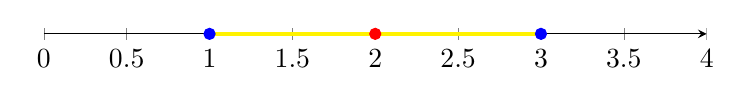
\begin{tikzpicture}
                \begin{axis}[
                  axis x line=middle,
                  axis y line = none,
                  xmin=0,
                  xmax=4,
                ]
                \addplot[red, only marks] 
                table {
                    2 0
                };
                \addplot[blue, only marks]
                table {
                    1 0
                    3 0
                };
                \addplot[yellow, very thick] coordinates {(1,0)(3,0)};
                \end{axis}
            \end{tikzpicture}
        \end{figure}
    \end{example}
    \begin{definition}
        Se $x_0 = +\infty$ un intorno di $x_0$ è un insieme del tipo $(a,+\infty),\;a\in\R$.\newline
        Un intorno di $x_0 = -\infty$ è un insieme del tipo $(-\infty, a),\;a\in\R$.
    \end{definition}
    \begin{definition}
        Data $A\subset\R \wedge x_0\overline{\R}$, $x_0$ si dice punto di accumulazione per $A$ se $\forall, U\, intorno\, di\, x_0.\; U\cup A-\{x_0\}\neq\emptyset$.\newline
        Vuol dire che "vicino" a $x_0$ ci sono altri punti di $A$ oltre a $x_0$ ($x_0$ potrebbe anche non appartenere ad $A$) 
    \end{definition}
    \begin{example}
        $A = (2,3),\; Acc(A) = \{\text{punti di accumulazione di A}\} = ?\quad x_0\in(2,3)$
        ongi intorno di $x_0$ interseca $A$ in infiniti punti.
        \begin{figure}[!htb]
            \centering
            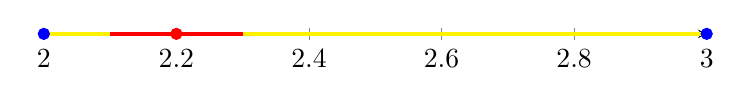
\begin{tikzpicture}
                \begin{axis}[
                  axis x line=middle,
                  axis y line = none,
                  xmin=2,
                  xmax=3,
                ]
                \addplot[red, only marks] 
                table {
                    2.2 0
                };
                \addplot[blue, only marks]
                table {
                    2 0
                    3 0
                };
                \addplot[yellow, very thick] coordinates {(2,0)(3,0)};
                \addplot[red, very thick] coordinates {(2.1,0)(2.3,0)};
                \end{axis}
            \end{tikzpicture}
        \end{figure}
    \end{example}
    \begin{definition}
        Un punto $x_0\in A$ si dice \underline{punto isolato} di $A$ se esiste un intorno $U$ di $x_0$ tale che $U\cup A = \{x_0\}$.
    \end{definition}
    \begin{example}
        $A = [2,3]\cap\{5\} \Rightarrow 5$ è punto isolato di $A$.
    \end{example}
    \begin{observation}
        Tutti gli elementi di $N$ sono punti isolati, quindi non ci sono punti di accumulazione.\newline
        $+\infty$ è l'unico punto di accumulazione per $N$.
    \end{observation}
    \begin{definition}
        $A\subset\R,\; x_0 \in A$ si dice punto interno ad $A$ se esiste $U$ intorno di $X_0$ tale che $U\subset A$. I punti interni si indicano con $int(A)$
    \end{definition}
    %Lezione 5 ottobre%
    \begin{definition}
        $A\subset\R,\;f:A\rightarrow\R$. Un punto $x_0\in A$ si dice punto di minimo locale (o relativo) se esiste un intorno $U$ di $x_0$ tale che $f(x)\geq f(x_0) \forall x\in U\cap A$
    \end{definition}
    \begin{definition}
        $A\subset\R,\;f:A\rightarrow\R$. Un punto $x_0\in A$ si dice punto di massimo locale (o relativo) se esiste un intorno $U$ di $x_0$ tale che $f(x)\leq f(x_0) \forall x\in U\cap A$
    \end{definition}
    Analogamente si definisco minimo locale stretto e massimo locale stretto.
    \begin{observation}
        Se $x_0$ è punto di minimo allora è anche punto di minimo locale.
    \end{observation}
    \newpage
    \subsection{Limite}
    \begin{definition}
        $A\subset\R,\;f:A\rightarrow\R ,\; x_0$ punto di accumulazione per $A$. Si dice che $l\in\overline{\R}$ è il limite per $x$ che tende ad $x_0$ di $f(x)$ se $\forall\, V\, intorno$ di $l\,\exists\, U$ intorno di $x_0.\; x\in U\cap A-\{x_0\}\Rightarrow f(x)\in V$.
    \end{definition}
    \[\lim_{x\rightarrow\ x_0} f(x) = l \Leftrightarrow \forall\, \varepsilon>0\;\exists\,\delta > 0.\; x\in A, |x-x_0| < \delta \wedge x\neq x_0 \Rightarrow |f(x)-l< \varepsilon\]
    \[\lim_{x\rightarrow +\infty} f(x) = l,\; l\in\R \Leftrightarrow \forall\,\varepsilon > 0.\; \exists\, a \in\R.\; x>a \Rightarrow |f(x)-l|< \varepsilon\]
    \[\lim_{x\rightarrow +\infty} f(x) = +\infty \Leftrightarrow \forall\, a \in\R.\; \exists\, b \in\R.\; x>b \Rightarrow f(x)> a\]
    (Analoghi i casi $l=-\infty \vee x_0 = -\infty$)
    \begin{observation}
        $f:A\rightarrow\R,\; A\subset\R,\,X_0\in A, x_0\in Acc(A)$. Allora $f$ è continua in $x_0 \Leftrightarrow \lim_{x\rightarrow X_0} f(x) = f(x_0)$ 
    \end{observation}
    \begin{observation}
        Una funzione è sempre continua nei punti isolati.
    \end{observation}
    \begin{observation}
        Nella definizione di limite non serve che $x_0$ sia nel dominio della funzione, basta che sia un punto di accumulazione per il dominio.
    \end{observation}
    \begin{example}
        \[f(x) = \frac{1}{x^2}\quad\lim_{x\rightarrow 0} f(x) = +\infty\]
        \begin{figure}[!htb]
            \centering
            \begin{tikzpicture}
                \begin{axis}[
                    axis lines = middle,
                    xmin = -3,
                    xmax = 3,
                    ymin = 0,
                    ymax = 10,
                    samples = 100
                ]
                    \addplot[blue, domain= -4:4] {1/x^2};
                    \addplot[red] coordinates {(-1,8)(1,8)};
                    \addplot[red,dashed] coordinates {(-0.35,8)(-0.35,0)};
                    \addplot[red,dashed] coordinates {(0.35,8)(0.35,0)};
                \end{axis}
            \end{tikzpicture}
        \end{figure}
    \end{example}
    \begin{theorem}[\textbf{Unicità del limite}]
        Se il limite esistw allora è unico.
    \end{theorem}
    \newpage
    \begin{definition}
        $A\subset\R ,\, x_0\in\R ,\, x_0\in Acc(A\cap[x_0,+\infty))\quad \func{f}{A}{\R}$ si dice che $l\in\Rext$ è il limite di $f(x)$ per $x$ che tende a $x_0$ da destra. E si scrive:
        \[\lim_{x\rightarrow x_0^+} f(x)=l\]
        Se $\forall\, V$ intorno di $l\; \exists\,\delta > 0. x_0<x<x_0+\delta , x\in A \Rightarrow f(x)\in V$.\newline
        Da sinisrtra se  
        Se $\forall\, V$ intorno di $l\; \exists\,\delta > 0. x_0-\delta <x<x_0\ , x\in A \Rightarrow f(x)\in V$ e sis scrive:
        \[\lim_{x\rightarrow x_0^-} f(x)=l\]
    \end{definition}
    \begin{example}
        \[
            f(x) = 
            \begin{cases}
                -1 \Rightarrow x<0 \\
                1 \Rightarrow x>0
            \end{cases}
            \quad \func{f}{(-\infty,0)\cup(0,+\infty)}{\R}\quad
            \begin{matrix}
                \lim_{x\rightarrow 0^+} f(x) & = & 1\\
                \lim_{x\rightarrow 0^-} f(x) & = & -1\\
            \end{matrix}
        \]
        \begin{figure}[!htb]
            \centering
            \begin{tikzpicture}
                \begin{axis}[
                    axis lines = middle,
                    xmin = -2,
                    xmax = 2,
                    ymin = -1.5,
                    ymax = 1.5
                ]
                    \addplot[red] coordinates {(0.05,1)(2,1)};
                    \addplot[red] coordinates {(-0.05,-1)(-2,-1)};
                \end{axis}
            \end{tikzpicture}
        \end{figure}
    \end{example}
    \begin{observation}
        $\lim_{x\rightarrow x_0} f(x) = l \Leftrightarrow \lim_{x\rightarrow x_0^-} f(x) = \lim_{x\rightarrow x_0^+} f(x) = l$.\newline
        Nell'esempio precedente non esiste limite in $x_0 = 0$ perché $\lim_{x\rightarrow 0^+} f(x) = 1 \neq \lim_{x\rightarrow 0^-} f(x) = -1$
    \end{observation}
    \newpage
    \begin{definition}
        $A\subset\R,\, \func{f}{A}{\R},\, x_0\in Acc(A)$ Si dice che $\lim_{x\rightarrow x_0} f(x) = l^+\; (l\in\R)$\newline 
        se esiste un intorno $U$ di $x_0$ tale che $x\in U\cap A-\{x_0\}\Rightarrow f(x)>l$\newline
        Si ha analogamente la definizione per $\lim_{x\rightarrow x_0} f(x) = l^-$
        \begin{plot}
            \begin{axis}[
                axis lines = middle,
                ymax = 5,
                ymin = 0,
                samples = 100
            ]
                \addplot[blue, domain= 0.1:5] {(1/x)+1};
                \addplot[red] coordinates {(0,1)(5,1)};
            \end{axis}
        \end{plot}
    \end{definition}
    \begin{example}
        \[f(x) = \frac{1}{x}\quad \Lim{x\to +\infty}{f(x)}{0^+}\]
        \begin{plot}
            \begin{axis}[
                axis lines = middle,
                samples = 100,
                ymax = 5,
                ymin = -5
            ]
                \addplot[red, domain= 0.1:5] {1/x};
                \addplot[red, domain= -0.1:-5] {1/x};
            \end{axis}
        \end{plot}
    \end{example}
    \newpage
    \begin{theorem}[\textbf{Permanenza del segno}]
        $A\subset\R,\, \func{f}{A}{\R},\, x_0\in Acc(A)$. Se esiste il $\Lim{x\to x_0}{f(x)}{l}\in\Rext \wedge l\neq0$ allora esiste un intorno $U$ di $x_0$ tale che se $x\in A\cap U-\{x_0\}$ allora $f$ ha lo stesso segno di $l$. 
    \end{theorem}
    \begin{example}
        \[\func{f}{(0,+\infty)}{\R}\quad f(x) = \frac{1}{x}\quad \Lim{x\to 0^+}{f(x)}{+\infty > 0} \Rightarrow f(x)>0 \text{ in un intorno destro di 0}\]
        \begin{plot}
            \begin{axis}[
                axis lines = middle,
                xmin = 0,
                xmax = 5,
                ymax = 5,
                ymin = 0,
                samples = 100
            ]
                \addplot[blue, domain=0.1:5] {1/x};
                \addplot[red, dashed, thick] coordinates {(0.5,0)(0.5,3)};
                \addplot[red, dashed, very thick] coordinates {(0.01,0)(0.01,3)};
                \addplot[red, very thick] coordinates {(0.01, 0)(0.5,0)};
                \node[red] at (110,30) {$f(x)>0$};
            \end{axis}
        \end{plot}
    \end{example}
    \begin{example}
        \textbf{Non} esiste $\lim_{x\to +\infty} \sin(x)$.\newline
        Se esistesse il limite $l\in\R$ allora scelgo $\varepsilon < \frac{1}{2}$ nella definizione di limite.
        Quindi dovrebbe esistere $a\geq 0$ t.c. $x>a\Rightarrow l-\varepsilon < \sin(x) < l+\varepsilon$. MA questo vorrebbe dire che $\sin(x)$ oscilla con un ampiezza minore di $2\varepsilon < 1$, mentre $\sin(x)$ oscilla con ampiezza 2.
        \begin{plot}
            \begin{axis}[
                axis lines = middle,
                xmin = -10,
                xmax = 10,
                ymin = -2,
                ymax = 2, 
                trig format plots=rad,
                samples=100
            ]

            \addplot[black, domain=-10:10] {sin(x)};
            \addplot[red] coordinates {(-10, 0.6)(10,0.6)};
            \addplot[red] coordinates {(-10, 0.4)(10,0.4)};
            \addplot[blue] coordinates {(-10, 0.5)(10,0.5)};
            \node[red] at (90,270) {$l+\varepsilon$};
            \node[red] at (90,230) {$l-\varepsilon$};
            \node[blue] at (110,260) {$l$};
            \end{axis}
        \end{plot}
    \end{example}
    \newpage
    \begin{example}
        \[
            f(x) = 
            \begin{cases}
                1 \Rightarrow x \geq 0 \\
                -1 \Rightarrow x < 0
            \end{cases}
            \quad
            \begin{matrix}
                \Lim{x\to 0^+}{f(x)}{1} & = & f(0) \\
                \Lim{x\to 0^-}{f(x)}{-1} & \color{red}\neq & \color{red}f(0) \\
            \end{matrix}
        \]
        \begin{plot}
            \begin{axis}[
                axis lines = middle,
                xmin = -3,
                xmax = 3,
                ymin = -1.5,
                ymax = 1.5,
                samples = 100
            ]
                \addplot[red, domain=0:3] {1};
                \addplot[red, domain=-0.01:-3] {-1};
                \addplot[red, only marks, very thick]
                table {
                    0 1
                };
            \end{axis}
        \end{plot}
    \end{example}
    \begin{definition}
        $A\subset\R ,\, x_0\in A,\, x_0\in Acc(A)$
        \begin{itemize}
            \item Se $\Lim{x\to x_0^+}{f(x)}{f(x_0)}$ allora si dice che $f$ è continua a dx in $x_0$.
            \item Se $\Lim{x\to x_0^-}{f(x)}{f(x_0)}$ allora si dice che $f$ è continua a sx in $x_0$.
        \end{itemize}
    \end{definition}
    \begin{observation}
        $f$ è continua in $x_0 \Leftrightarrow$ è continua in sia a destra che a sinistra in $x_0$.
    \end{observation}
    \begin{theorem}[\textbf{Teorema del confronto}]
        $A\subset\R,\, x_0\in Acc(A),\, \func{f\circ g}{A}{\R}$. Se esistono $\Lim{x\to x_0}{f(x)}{l_1} \wedge \Lim{x_to x_0}{g(x)}{l_2}$ e se esiste $U$ intorno di $x_0$ tale che $x\in U\cap A-\{x_0\}\Rightarrow f(x)\leq g(x)$ allora $l_1 \leq l_2$.
        \begin{plot}
            \begin{axis}[
                axis lines = middle,
                xmin = 0,
                xmax = 4,
                ymax = 5,
                ymin = 0,
                samples = 100 
            ]
                \addplot[blue, domain=0.5:5] {(1/x)+1};
                \addplot[red, domain=0.5:5] {(1/x)+2};
                \addplot[blue, dashed] {1};
                \addplot[red, dashed] {2};
            \end{axis}
        \end{plot}
    \end{theorem}
    Sinteticamente si potrebbe dire che la disuguaglianza passa al al limite (nelle ipotesi corrette):
    \[f(x) \leq g(x)\Rightarrow \lim_{x\to x_0} f(x) \leq \lim_{x\to x_0} g(x)\]
    \newpage
    \begin{observation}
        Se fosse $f(x) < g(x)$ potrei concludere $\lim_{x\to x_0} f(x) < \lim_{x\to x_0} g(x)$? \textbf{\color{red}NO!}
    \end{observation}
    \begin{example}
        \[\color{red}f(x) = -\frac{1}{x} \quad \color{blue} g(x) = \frac{1}{x}\quad \color{black} f(x)<g(x) \text{ ma} \lim_{x\to +\infty}f(x) = \lim_{x\to +\infty} g(x) = 0\]
        \begin{plot}
            \begin{axis}[
                axis lines = middle,
                xmin = 0,
                xmax = 5,
                ymin = -4,
                ymax = 4,
            ]
                \addplot[red, domain= 0.1:5] {-(1/x)};
                \addplot[blue, domain= 0.1:5] {(1/x)};
            \end{axis}
        \end{plot}
    \end{example}
    Le disuguaglianze passano al limite, ma diventano deboli:
    \[f(x) < g(x)\Rightarrow \lim_{x\to x_0} f(x) \leq \lim_{x\to x_0} g(x)\]
    \begin{theorem}[\textbf{Teorema dei Carabinieri}]
        $A\subset\R,\, x_0\in Acc(A),\; \func{f,g,h}{A}{\R}$ Se esistono $\Lim{x\to x_0}{f(x)}{l} \wedge \Lim{x\to x_0}{h(x)}{l}$ e se esiste un intorno $U$ di $x_0$ t.c. $x\in A\cap U-\{x_0\} \Rightarrow f(x)\leq g(x) \leq h(x)$ allora esiste $\Lim{x\to x_0}{g(x)}{l}$
        \begin{plot}
            \begin{axis}[
                axis lines = middle,
                trig format plots=rad,
                xmin = 0, 
                xmax = 100,
                ymin = 0,
                ymax = 2,
                samples = 1000
            ]

                \addplot[green, domain= 0.1:100] {(sin(x)/x)+1};
                \addplot[orange, domain= 0.1:100] {(1/x)+1};
                \addplot[blue, domain= 0.1:100] {-(1/x)+1};
                \addplot[red, domain= 0:100] {1};
            \end{axis}
        \end{plot}
    \end{theorem}
    Dall'esistenza dei limiti di $f,h$ (uguali fra loro) deduco l'esistenza del limite di $g$.
    \newpage
    \begin{theorem}[Somma e Prodotto]
        $A\subset\R,\, x_0\in Acc(A),\; \func{f\circ g}{A}{\R}$ Supponiamo che esistono i limiti $\Lim{x\to x_0}{f(x)}{l_1} \wedge \Lim{x\to x_0}{g(x)}{l_2}$, con $l_1,l_2\in\Rext$:
        \begin{enumerate}
            \item Se ha senso $l_1+l_2 \Rightarrow \Lim{x\to x_0}{(f+g)(x)}{l_1+l_2}$
            \item Se ha senso $l_1*l_2 \Rightarrow \Lim{x\to x_0}{(f*g)(x)}{l_1*l_2}$
        \end{enumerate}
        Sono esclusi i casi:
        \begin{enumerate}
            \item $l_1 = +\infty \wedge l_2 = -\infty$ (e viceversa) per la Somma.
            \item $(l_1 = +\infty \wedge l_2 = 0) \vee (l_1 = -\infty \wedge l_2 = 0)$ (e viceversa) per il Prodotto.
        \end{enumerate}
        E si dicono \underline{Forme di indeterminazione}.
    \end{theorem}
    \begin{example}
        Perché non ha senso $(+\infty) + (-\infty)$?
        \[f(x) = 2x,\; g(x) = -x\quad\Lim{x\to +\infty}{f(x)}{+\infty},\, \Lim{x\to +\infty}{g(x)}{-\infty}\Rightarrow \Lim{x\to +\infty}{2x-x}{\Lim{x\to +\infty}{x}{+\infty}}\]
        Allora in questo caso avrei che $(+\infty) + (-\infty) = +\infty$\newline
        Invece se prendo:
        \[f(x) = \frac{x}{2},\,g(x) = -x\quad \Lim{x\to +\infty}{f(x)}{+\infty},\,\Lim{x\to +\infty}{g(x)}{-\infty} \Rightarrow \Lim{x\to +\infty}{\frac{x}{2}-x}{\Lim{x\to +\infty}{-\frac{x}{2}}{-\infty}}\]
        E in questo caso avei $(+\infty) + (-\infty) = -\infty$. Quale delle due scelgo?\newline
        Per questo motivo dico che $(+\infty) + (-\infty)$ non ha senso. Analogamente per il prodotto $0*(+\infty)$
    \end{example}
    \begin{theorem}
        $A\subset\R,\, x_0\in Acc(A),\,\func{f}{A}{\R}$ Se esiste $\Lim{x\to x_0}{f(x)}{l} \wedge l\in \R\; (l\neq\pm\infty)$. Allora $l$ è limitata in un intorno di $x_0$ cioè $\exists\, U\, di\, x_0 \wedge M\in\R,\, M>0\; t.c\; x\in U\cap A\Rightarrow |f(x)| \leq M$
    \end{theorem}
    \begin{example}
        $f(x) = \frac{1}{x}$ è limitata in un intorno di $+\infty$ perché $\Lim{x\to +\infty}{f(x)}{0}$
        \begin{plot}
            \begin{axis}[
                axis lines = middle,
                xmin = 0,
                xmax = 10,
                ymax = 4,
                samples = 200
            ]
                \addplot[blue, domain= 0.1:10] {1/x};
                \addplot[red, domain= 0:10] {0.3};
                \node[red] at (5,35) {M};
            \end{axis}
        \end{plot}
    \end{example}
    \newpage
    \begin{definition}
        Notazioni per limiti:
        \begin{itemize}
            \item Se $\Lim{x\to x_0}{f(x)}{0}$ allora si dice che $f$ è infinitesima per $x$ che tende ad $x_0.$
            \item Se $\Lim{x\to x_0}{f(x)}{+\infty}$ allora si dice che $f$ diverge positivamente per $x$ che tende ad $x_0.$
            \item Se $\Lim{x\to x_0}{f(x)}{-\infty}$ allora si dice che $f$ diverge negativamente per $x$ che tende ad $x_0.$
            \item Se $\Lim{x\to x_0}{f(x)}{l},\, l\in\R\,(finito)$ allora si dice che $f$ converge a $l$ per $x$ che tende ad $x_0.$
        \end{itemize}
    \end{definition}
    \begin{proposition}
        Se $f$ è limitata inferiormente in un intorno di $x_0$ e $\Lim{x\to x_0}{g(x)}{+\infty}\Rightarrow \Lim{x\to x_0}{(f+g)(x)}{+\infty}$.\newline
        Se $f$ è limitata superiormente in un intorno di $x_0$ e $\Lim{x\to x_0}{g(x)}{-\infty}\Rightarrow \Lim{x\to x_0}{(f+g)(x)}{-\infty}$.\newline
        Se $f$ è limitata in un intorno di $x_0$ e $\Lim{x\to x_0}{g(x)}{0} \Rightarrow \Lim{x\to x_0}{(f*g)(x)}{0}$.\newline
        \color{red} Sono tutte conseguenze del Teorema dei Carabinieri.
    \end{proposition}
    %Lezione 7 Ottobre%
    \begin{proposition}
        Se $\Lim{x\to x_0}{f(x)}{0^+} \Rightarrow \Lim{x\to x_0}{\frac{1}{f(x)}}{+\infty}$.\newline
        Se $\Lim{x\to x_0}{f(x)}{0^-} \Rightarrow \Lim{x\to x_0}{\frac{1}{f(x)}}{-\infty}$.\newline
        Se $\Lim{x\to x_0}{f(x)}{+\infty} \Rightarrow \Lim{x\to x_0}{\frac{1}{f(x)}}{0^+}$.\newline
        Se $\Lim{x\to x_0}{f(x)}{-\infty} \Rightarrow \Lim{x\to x_0}{\frac{1}{f(x)}}{0^-}$.\newline
        Se $\Lim{x\to x_0}{f(x)}{l},\; l\neq 0,\pm\infty \Rightarrow \Lim{x\to x_0}{\frac{1}{f(x)}}{\frac{1}{l}}$.\newline
    \end{proposition}
    \begin{proposition}
        $a,b\in\Rext,\, \func{f}{(a,b)}{\R}$ con $f$ debolmente crescente. Allora esistono:
        \[\Lim{x\to a^+}{f(x)}{inf_{x\in(a,b)}(f(x))} \wedge \Lim{x\to b^-}{f(x)}{sup_{x\in(a,b)}(f(x))}\]
        Analogo risultato se $f$ è debolmente decrescente.
    \end{proposition}
    \begin{example}
        \[\func{f}{(2,3)}{\R},\; f(x) = x^2 - \frac{3}{2}x\]
        \begin{plot}
            \begin{axis}[
                axis lines = middle,
                xmin = 0,
                xmax = 5,
                ymin = 0,
                ymax = 10,
                samples = 100
            ]
                \addplot[blue, domain=2:4] {(x^2)-(1.5*x)};
                \addplot[red, dashed] coordinates {(0,10)(4,10)};
                \addplot[red, dashed] coordinates {(0,1)(2,1)};
            \end{axis}
        \end{plot}
    \end{example}
    \newpage
    \subsection{Limiti Fondamentali}
    \begin{itemize}
        \item $\Lim{x\to +\infty}{x^n}{+\infty}\quad \forall\, n\in N$
        \item $\Lim{x\to +\infty}{\frac{1}{x^n}}{0}\quad \forall\, n\in N$
        \item $\Lim{x\to +\infty}{e^x}{+\infty}$
        \item $\Lim{x\to -\infty}{e^x}{0^+}$
        \item $\Lim{x\to 0^+}{\log(x)}{-\infty}$
        \item $\Lim{x\to +\infty}{\log(x)}{+\infty}$
    \end{itemize}
    \subsection{Limiti di polinomi}
    $p(x) = a_nx^n + a_{n-1}x^{n-1} + \dots + a_1x + a_0$\newline
    $\Lim{x\to +\infty}{a_nx^n + a_{n-1}x^{n-1} + \dots + a_1x + a_0}{\lim_{x\to +\infty}a_nx^n}$
    \begin{example}
        \[\Lim{x\to -\infty}{-2x^5+3x^2}{\Lim{x\to -\infty}{-2x^5}{\Lim{x\to -\infty}{-2(-\infty)^5}{-2(-\infty) = +\infty}}}\]
    \end{example}
    \subsection{Limiti di funzioni razionali}
    $f(x) = \frac{p(x)}{q(x)}$\newline
    $\Lim{x\to\pm\infty}{\frac{p(x))}{q(x)}}{\Lim{x\to\pm\infty}{\frac{a_nx^n + a_{n-1}x^{n-1} + \dots + a_1x + a_0}{b_mx^m + b_{m-1}x^{m-1} + \dots + b_1x + b_0}}{\lim_{x\to\pm\infty}\frac{a_nx^n}{b_mx^m}}}$
    \begin{example}
        \[\Lim{x\to +\infty}{\frac{7x^4+5x^2}{-2x^3}}{\Lim{x\to +\infty}{\frac{7x^4}{-2x^3}}{\Lim{x\to +\infty}{\frac{7x}{-2}}{-\infty}}}\]
    \end{example}
    \subsection{Limiti Notevoli}
    Limiti notevoli per $x\to 0$:
    \begin{itemize}
        \item $\Lim{x\to 0}{\frac{\sin(x)}{x}}{1}$
        \item $\Lim{x\to 0}{\frac{1-\cos(x)}{x^2}}{\frac{1}{2}}$
        \item $\Lim{x\to 0}{\frac{e^x-1}{x}}{1}$
        \item $\Lim{x\to 0}{\frac{\log(1+x)}{x}}{1}$
    \end{itemize}
    \subsection{Limiti della composizione di funzioni}
    \begin{theorem}
        $A,B,C\in\R ,\, \func{f}{A}{B}\;\func{g}{B}{C}, x_0\in Acc(A),\, \Lim{x\to x_0}{f(x)}{y_0} \wedge\; y_0\in Acc(B) \wedge \exists \Lim{y\to y_0}{g(x)}{l}\in\overline{\R}$ e se vale almeno una delle ipotesi:
        \begin{itemize}
            \item $y_0\in B \wedge g$ è continua in $y_0$
            \item $\exists U$ intorno di $x_0$ tale che se $x\in U\cap A-\{x_0\}\Rightarrow f(x)\neq y_0$ 
        \end{itemize}
        Allora $\Lim{x\to x_0}{(g\circ f)(x)}{l}$
    \end{theorem}
    %Lezione 8 ottobre pagina 20
\end{document}